\section[Plus d'humains, plus de chats, moins de machines]{Plus d'humains, plus de chat, moins de machines}

\subsection{Moins d'algorithmes et plus de contact entre humain}

\begin{frame}{Des acteurs pour des internets plus respectueux (1/2)}
  \begin{center}
    
\includegraphics[height=0.8\textheight]{un_autre_internet/les_fai_dont_vous_etes.pdf}
  \end{center}
\end{frame}

\begin{frame}{Des acteurs pour des internets plus respectueux (2/2)}
  \begin{columns}
    \begin{column}{0.5\textwidth}
      \begin{tabular}{cccc}
        
\includegraphics[width=0.24\textwidth]{un_autre_internet/hadoly.png} &
        \begin{tikzpicture}
          \node (img1) at (0,0) {
\includegraphics[width=0.24\textwidth]{un_autre_internet/arn.png}};
          \node (img2) at (0, -1) {
\includegraphics[width=0.24\textwidth]{un_autre_internet/outils_conviviaux.png}};
        \end{tikzpicture} &
        
\includegraphics[width=0.24\textwidth]{un_autre_internet/tux_family.png} &
        
\includegraphics[width=0.24\textwidth]{un_autre_internet/framasoft.png}  \\
        
\includegraphics[width=0.24\textwidth]{un_autre_internet/marsnet.png} &
        
\includegraphics[width=0.24\textwidth]{un_autre_internet/devloprog.png} &
        
\includegraphics[width=0.24\textwidth]{un_autre_internet/3hg.png} &
        
\includegraphics[width=0.24\textwidth]{un_autre_internet/artifaille.png} \\
      \end{tabular}
    \end{column}
    \begin{column}{0.5\textwidth}
    \begin{center}
      \includegraphics[height=0.8\textheight]{un_autre_internet/chatons.png}
    \end{center}
    \end{column}
  \end{columns}
\end{frame}

\begin{frame}{Des volontés communes}
  \begin{columns}
    \begin{column}{0.4\textwidth}
      \begin{itemize}
        \item La neutralité du net
        \item La transparence
        \item L'humain au centre
        \item Rester local
      \end{itemize}
    \end{column}
    \begin{column}{0.6\textwidth}
      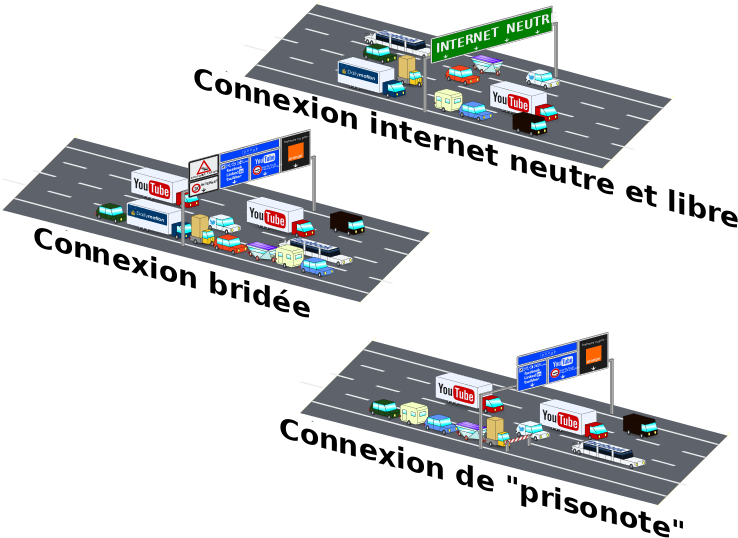
\includegraphics[width=0.4\textwidth]{un_autre_internet/autoroute.png}
      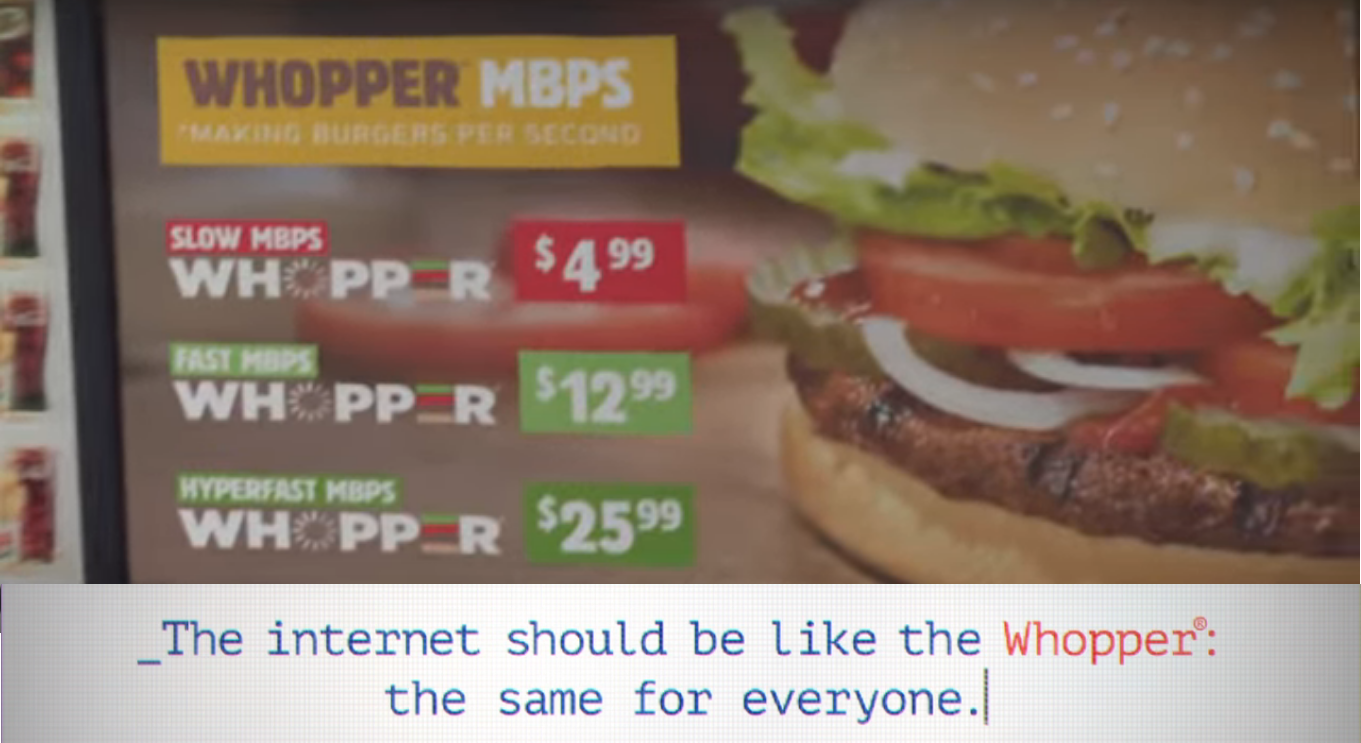
\includegraphics[width=0.4\textwidth]{un_autre_internet/whopper.png} \\
      
\includegraphics[width=0.4\textwidth]{un_autre_internet/local.png}
      
\includegraphics[width=0.4\textwidth]{un_autre_internet/groupetravail.png}
    \end{column}
  \end{columns}
\end{frame}

\subsection{Les CHATONS: Hadoly}

\begin{frame}{Hadoly: Hébergeur Associatif Décentralisé et Ouvert à Lyon}
  \begin{columns}
    \begin{column}{0.5\textwidth}
      \centering
      
\includegraphics[width=0.5\textwidth]{un_autre_internet/hadoly.png}\\
      https://hadoly.fr/
    \end{column}
    \begin{column}{0.5\textwidth}
      \begin{itemize}
        \item Services ouverts à tous
        \begin{itemize}
            \item Pads
            \item Wiki
            \item Docs
            \item PostIt
        \end{itemize}
        \item Services aux adhérents
        \begin{itemize}
          \item Mail
          \item Cloud
          \item Git
          \item Projets
        \end{itemize}
      \end{itemize}
    \end{column}
  \end{columns}
\end{frame}

\begin{frame}{Hadoly: Des services ouverts à tous}
  \centering
  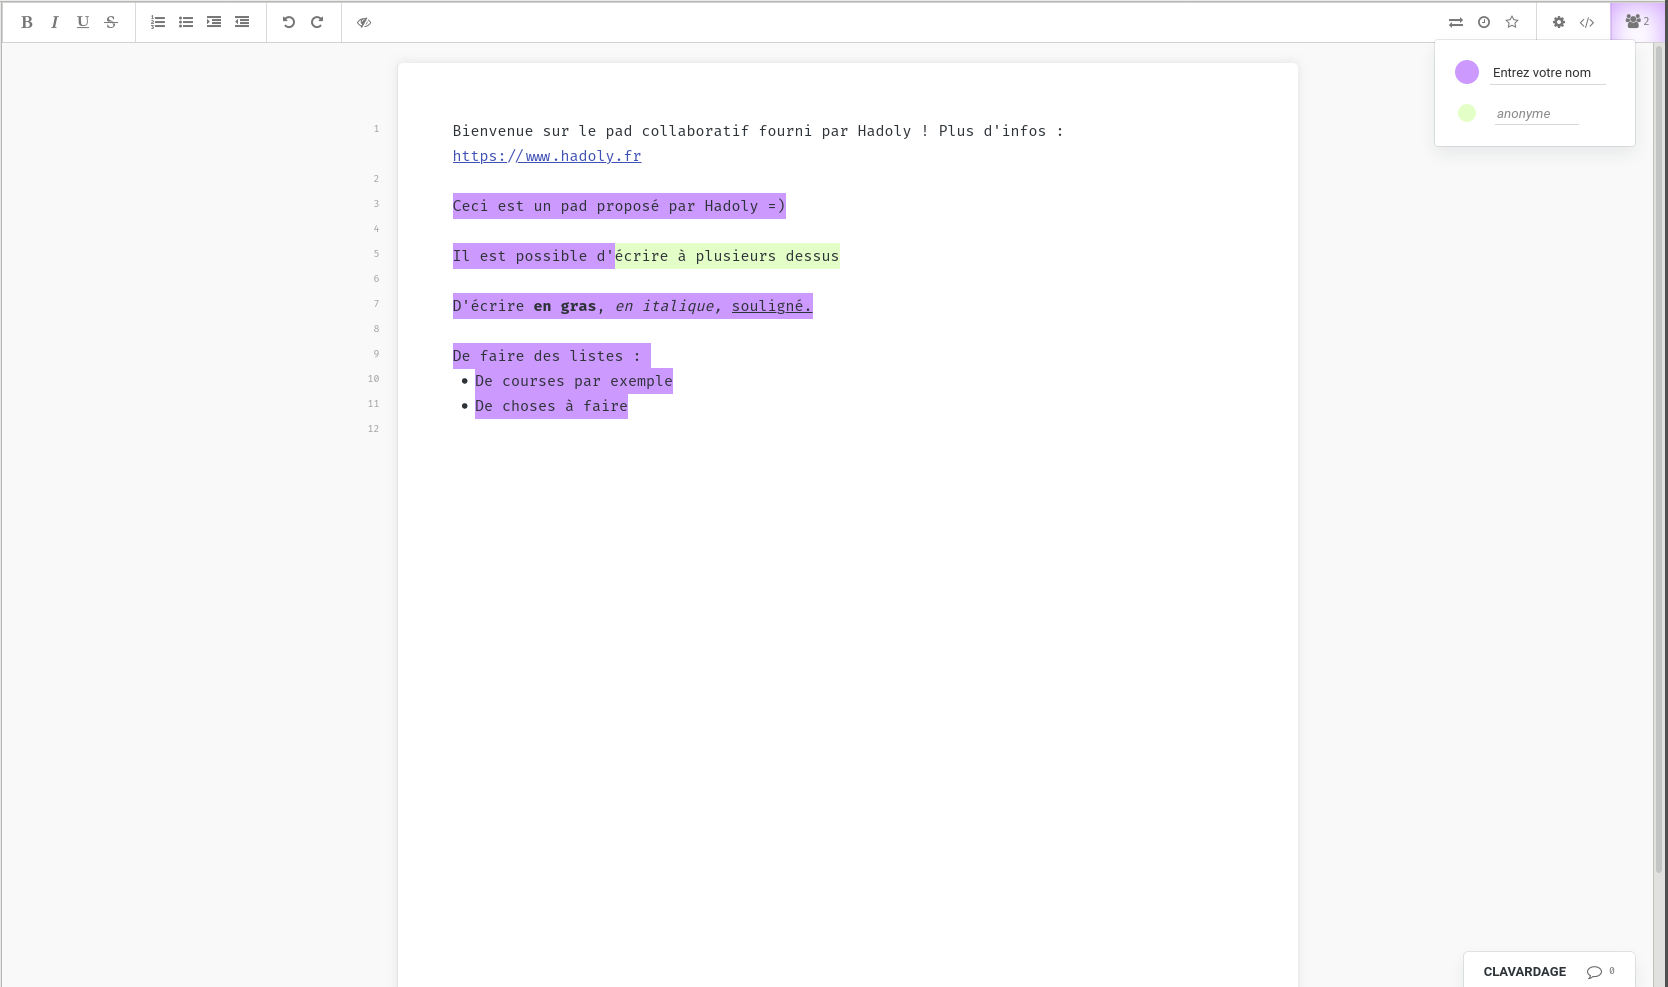
\includegraphics[width=0.8\textwidth]{un_autre_internet/pad_hadoly.png}\\
\end{frame}

\begin{frame}{Hadoly: C'est aussi des mails}
  \centering
  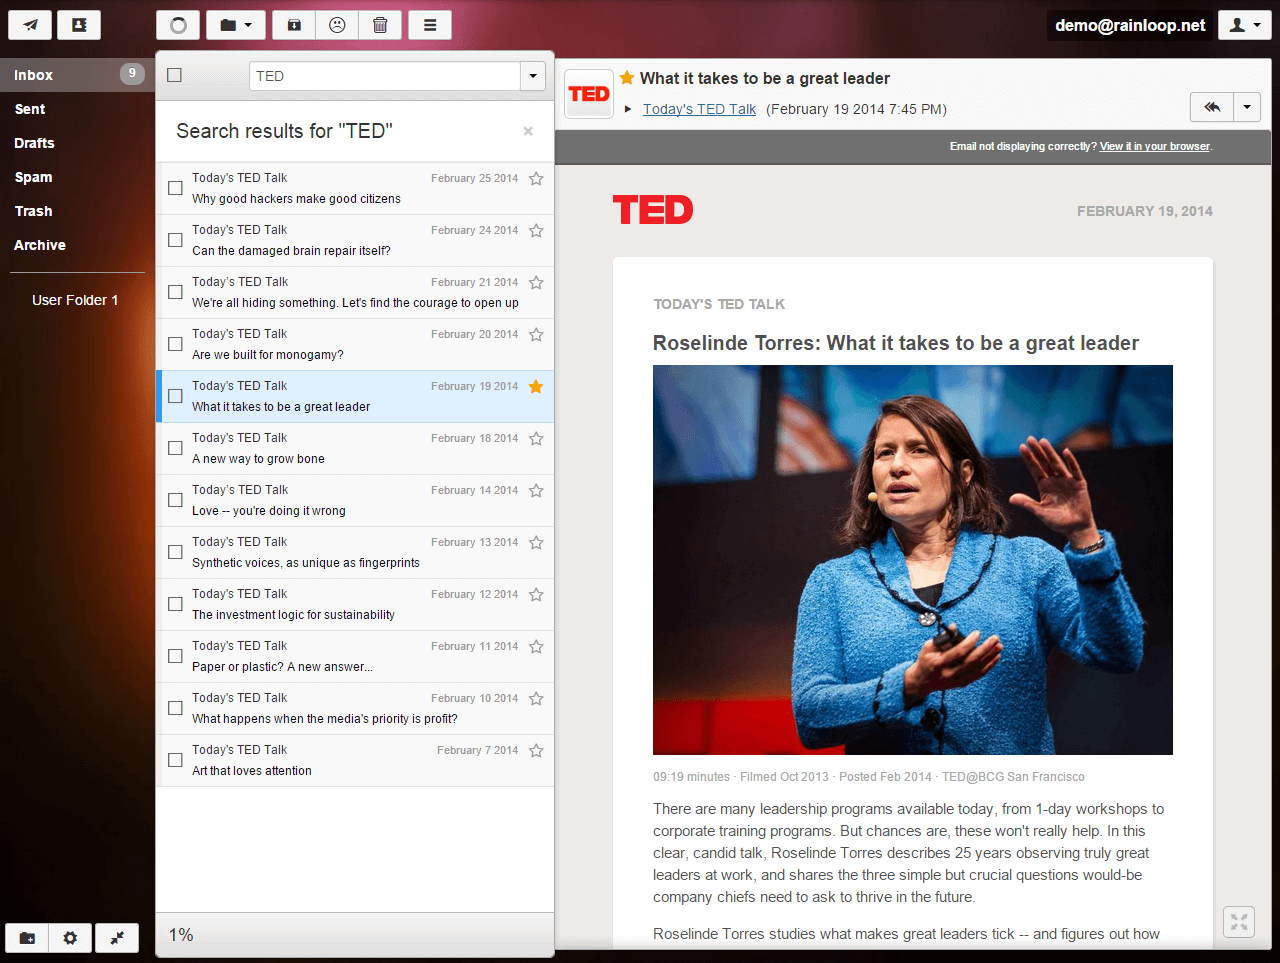
\includegraphics[width=0.8\textwidth]{un_autre_internet/rainloop.png}\\
  \tiny Image presque contractuelle.
\end{frame}

\begin{frame}{Hadoly: Un espace de stockage en ligne ("cloud")}
  \centering
  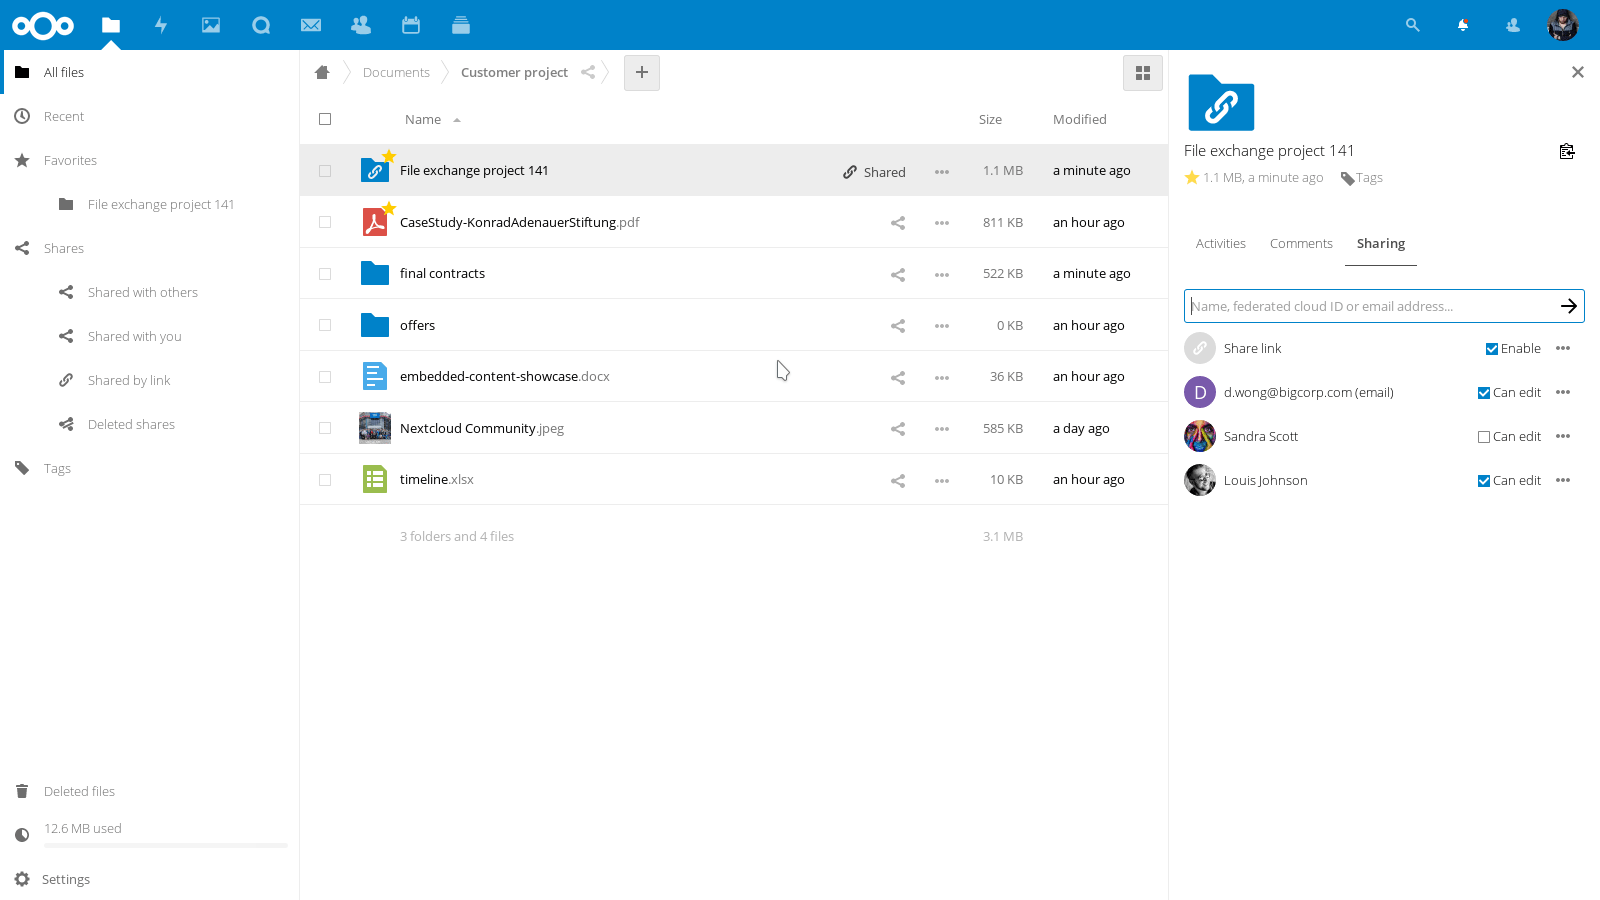
\includegraphics[width=0.8\textwidth]{un_autre_internet/nextcloud.png}\\
  \tiny Image presque contractuelle.
\end{frame}

\begin{frame}{Hadoly: Et bien d'autres}
  \centering
  \begin{tikzpicture}
    \node (img1) {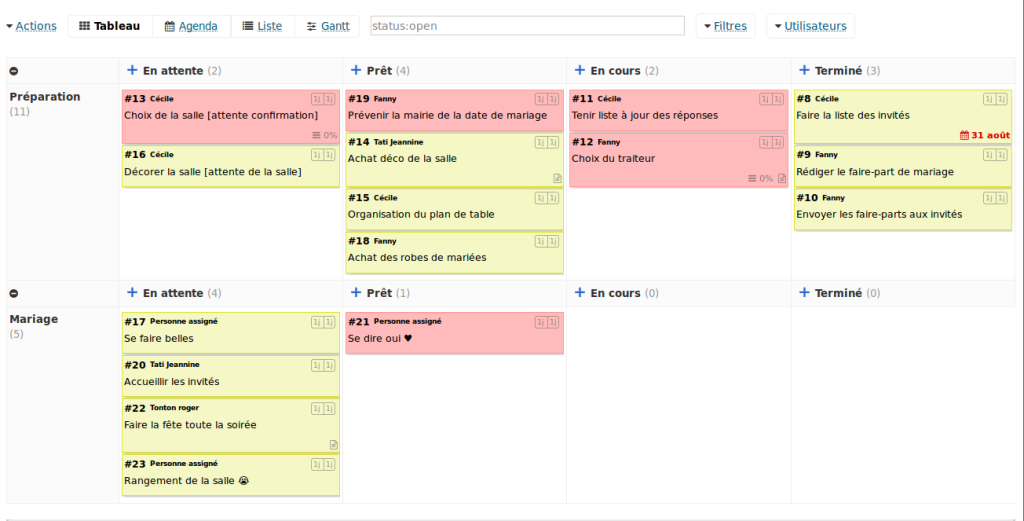
\includegraphics[width=0.7\textwidth]{un_autre_internet/kanboard.png}};
    \node (img2) at (img1.south east) {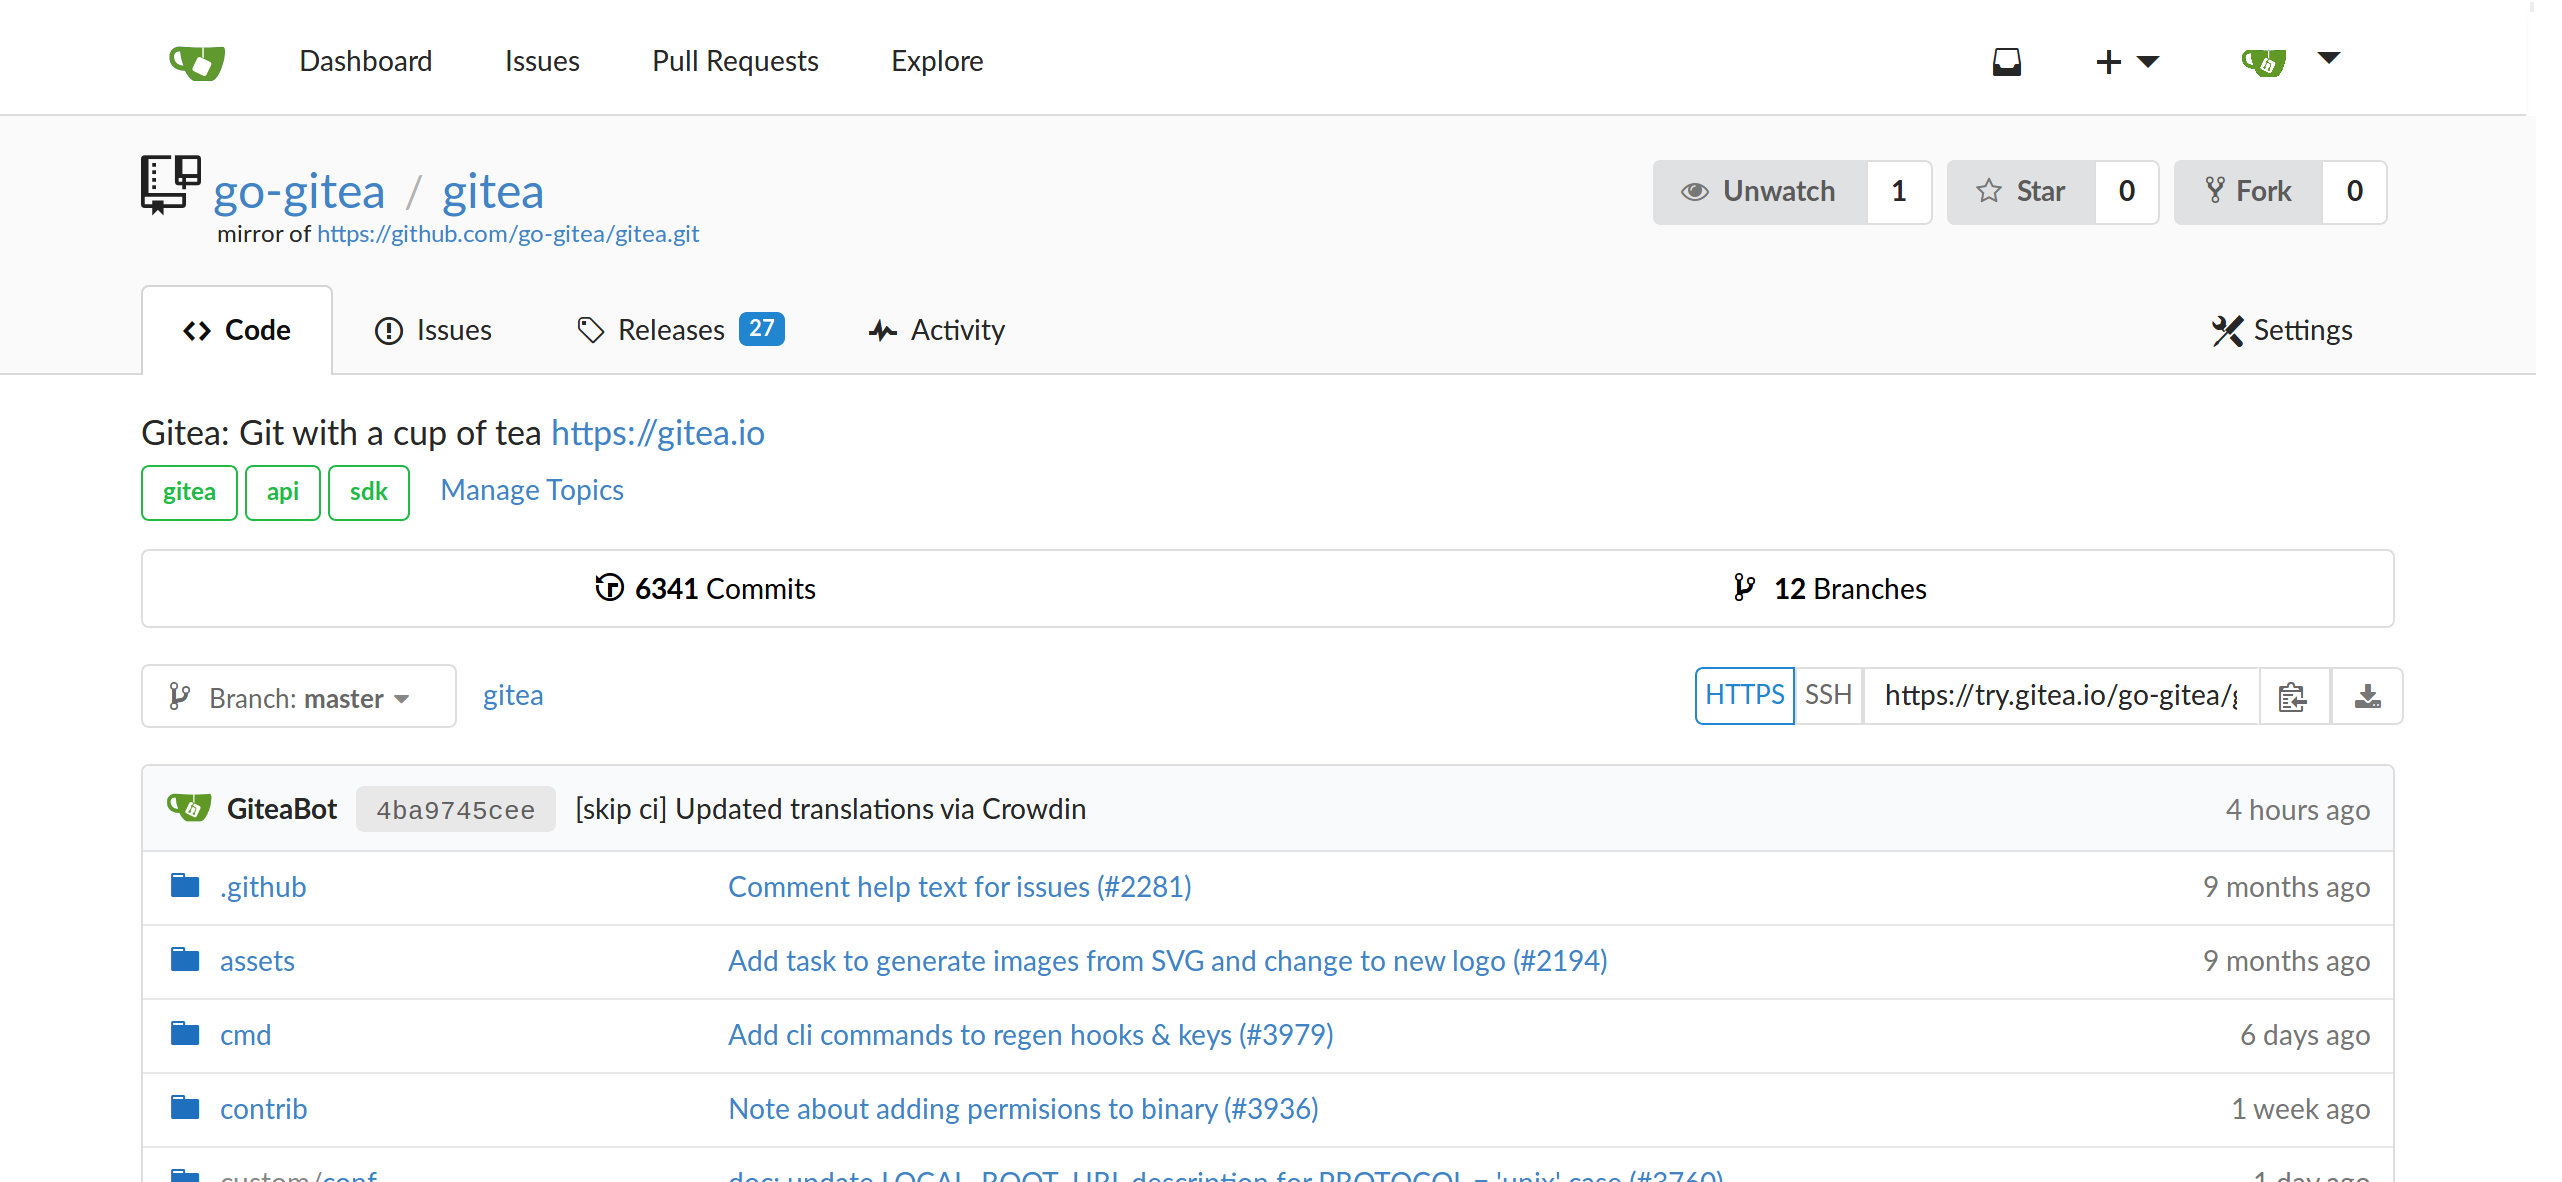
\includegraphics[width=0.7\textwidth]{un_autre_internet/gitea.png}};
  \end{tikzpicture}\\
  \tiny Images presque contractuelles.
\end{frame}

\subsection{Les FAI Associatif: Illyse}

\begin{frame}{Illyse: Internet Libre sur Lyon et Saint-Etienne}
  \begin{columns}
    \begin{column}{0.5\textwidth}
      \centering
      
\includegraphics[width=0.8\textwidth]{un_autre_internet/illyse.png}\\
      https://www.illyse.net/
    \end{column}
    \begin{column}{0.5\textwidth}
      \begin{itemize}
        \item De l'xDSL
        \item Des VPNs
        \item De l'internet par onde radio
        \item De la fibre \\{\tiny(pour l'instant, dans la Loire)}
      \end{itemize}
    \end{column}
  \end{columns}
\end{frame}

\begin{frame}{Illyse: De l'xDSL ...}
  \centering
  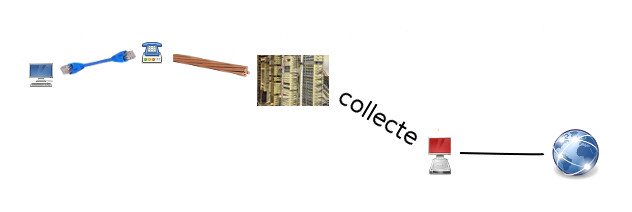
\includegraphics[width=0.8\textwidth]{un_autre_internet/adsl.png}
\end{frame}

\begin{frame}{Illyse: \hfill ... Du VPN ...\hfill}
  \centering
  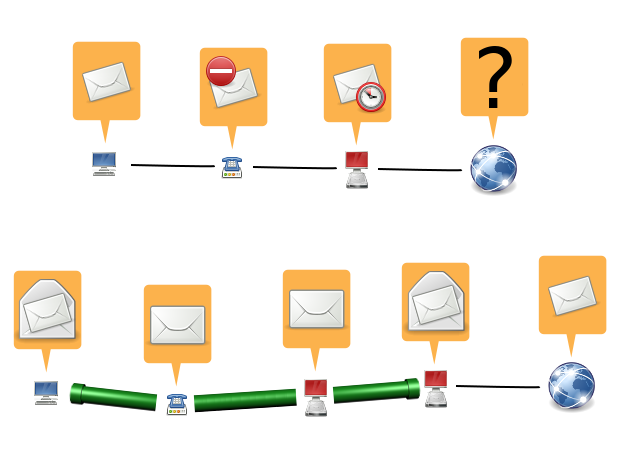
\includegraphics[width=0.8\textwidth]{un_autre_internet/vpn.png}
\end{frame}

\begin{frame}{Illyse: \hfill ... De l'internet par onde radio ...\hfill}
  \centering
  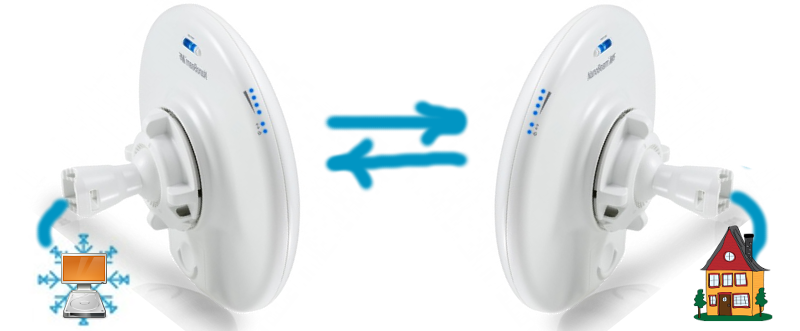
\includegraphics[width=0.8\textwidth]{un_autre_internet/antennes.png}
\end{frame}

\begin{frame}{Illyse: \hfill ... Et de la fibre (1/2)}
  \begin{columns}
    \begin{column}{0.5\textwidth}
      \centering
      
\includegraphics[width=0.4\textwidth]{un_autre_internet/fibre_1.png}
      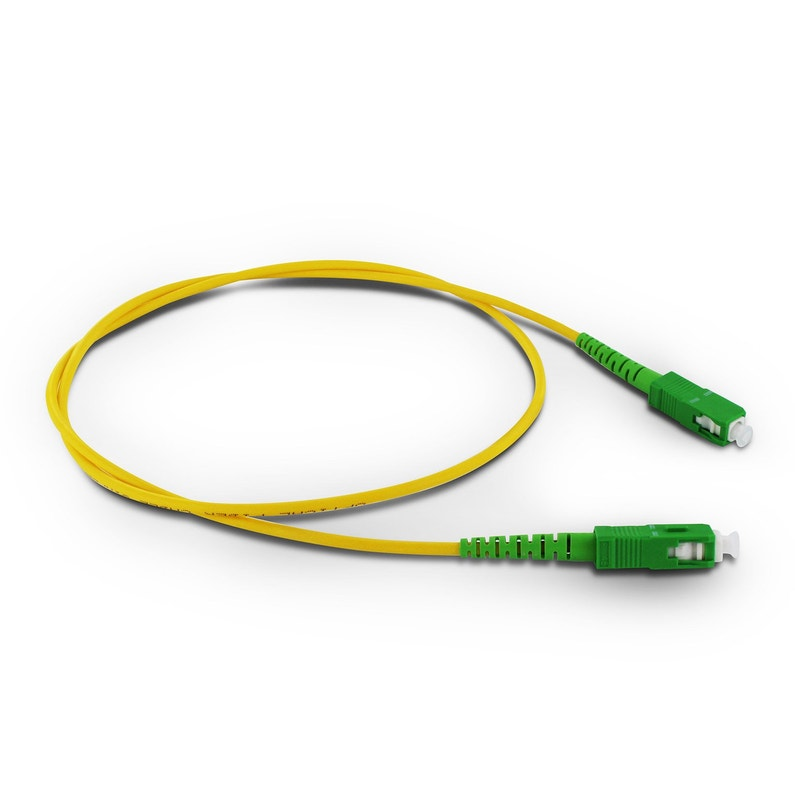
\includegraphics[width=0.4\textwidth]{un_autre_internet/fibre_2.png}\\
      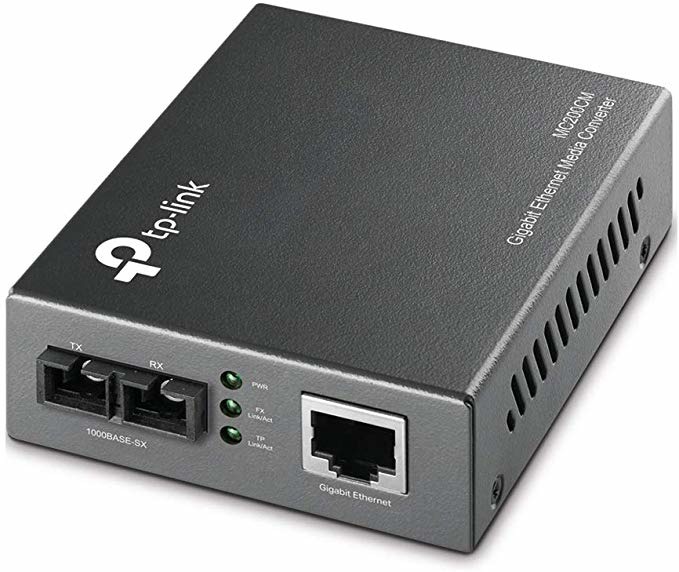
\includegraphics[width=0.4\textwidth]{un_autre_internet/fibre_3.png}
    \end{column}
    \begin{column}{0.5\textwidth}
      \centering
      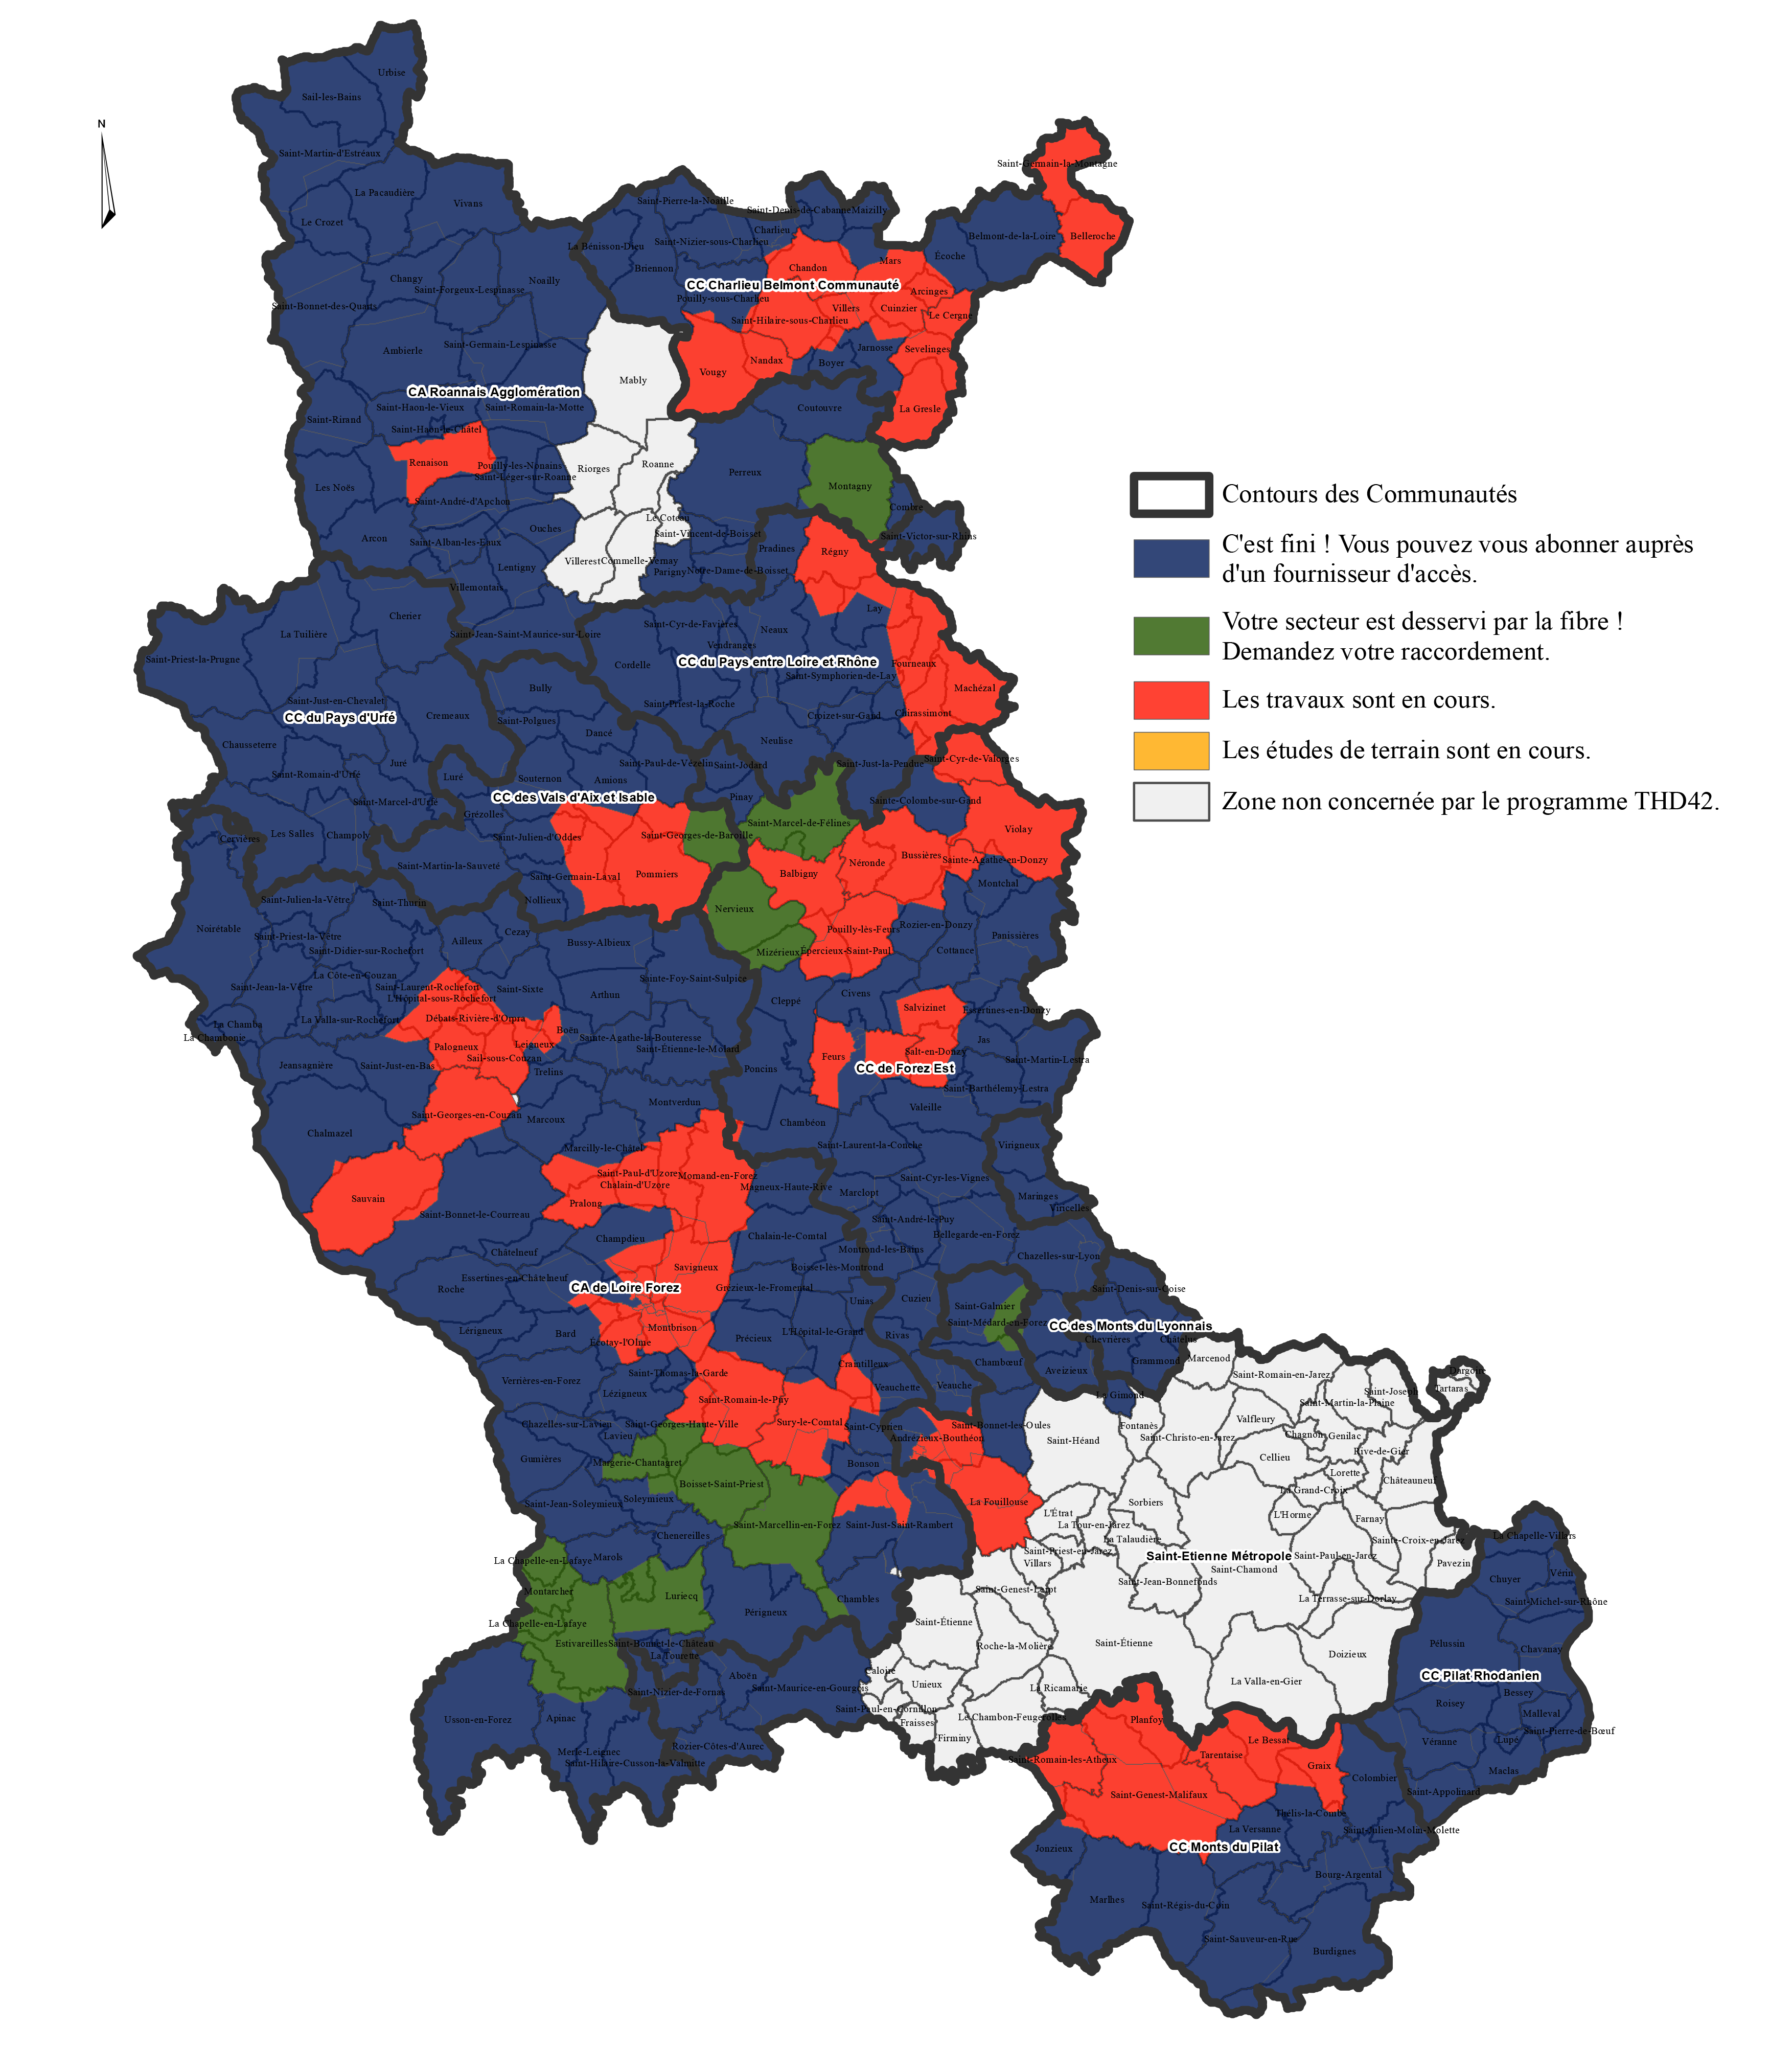
\includegraphics[width=\textwidth]{un_autre_internet/fibre_zone_dense.png}
    \end{column}
  \end{columns}
\end{frame}

\begin{frame}{Illyse: \hfill ... Et de la fibre (2/2)}
  \centering
  Donc si j'habite dans la loire ?
  
\includegraphics[width=0.8\textwidth]{un_autre_internet/fibre_yeah.png} \\
  Sinon, malheureusement, il va falloir attendre.
\end{frame}


\begin{frame}{Convaincu·e·s ? Alors rejoignez-nous}
  \centering
  Faisons des internets un monde plus humains, \\
  mais avec toujours autant de chats !

  
\includegraphics[height=0.7\textheight]{un_autre_internet/adoptez_les.png}
\end{frame}

% vim: ts=2: sw=2: sts=2
